\subsection{Einordnung im Standardmodell der Elementarteilchen}

\begin{iframe}
	\begin{figure}
		\centering
		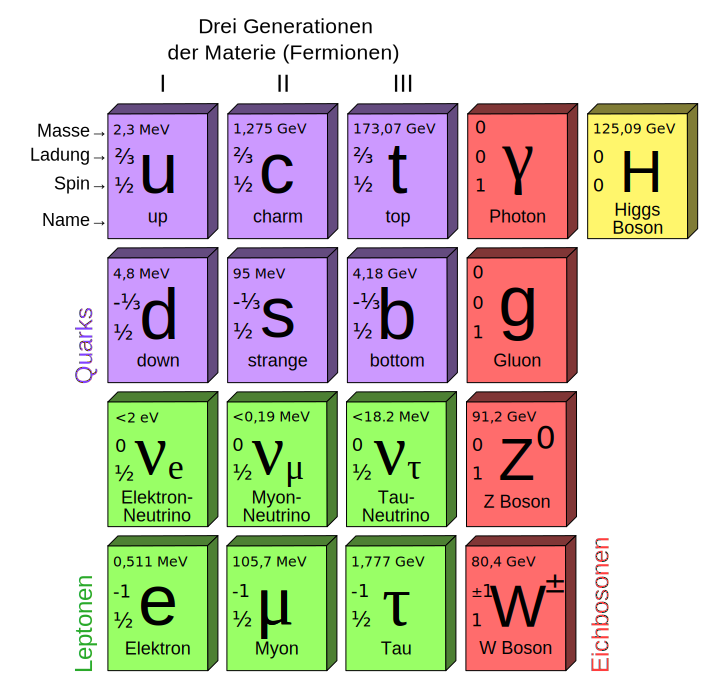
\includegraphics[width=5.5cm]{img/standardmodel}
		\caption{Standardmodell\cite{standardmodel}}
	\end{figure}
	
\end{iframe}
\note[itemize]{
	\item Eichboson und Elementarteilchen
	\item schwache WW
	\item eigenes Antiteilchen
	\item W+- => elek. Teilchen WW (beta Zerfall)
	\item Z0 => auch neutral Teilchen WW (Neutrino)
}
\subsection{Elektroschwache Vereinheitlichung}
\subsection{Zerfallsbreite}